\documentclass[a4paper,10pt]{article}
\usepackage[utf8]{inputenc}
\usepackage[T1]{fontenc}
\usepackage[frenchb]{babel}
\usepackage{numprint}
\usepackage{graphicx}

%opening
\title{Apprentissage par des réseaux de neurones}
\author{E. Beghdadi, M. Marrakchi Benazzouz, T. Chabal, Y. Vanlaer, T. Giraudon}

\begin{document}

\maketitle

\begin{abstract}

\end{abstract}

\section{Introduction}
En 1963, l'Américain Donald Michie créé Menace, \textit{Machine Educable Noughts And Crosses Engine},
une machine capable de rivaliser avec des joueurs humains au jeu du Tic-Tac-Toe, plus connu en France sous le nom de morpion.
Pour réaliser cette prouesse technologique, il utilise alors la technique de \textit{l'apprentissage par renforcement}.
Celle-ci consiste à faire jouer la machine un grand nombre de fois contre un joueur réel et à apprendre de ces parties
en corrigeant sa stratégie au fur et à mesure. Cette réussite signe alors la naissance du machine learning tel que
nous le connaissons aujourd'hui. \\
Dans les années 1970-1980, beaucoup de progrès théoriques sont réalisés : on imagine ainsi un système
directement inspiré du vivant, le réseau de neurones. Celui-ci consiste en un agencement de couches de neurones successives,
appelés les \textit{layers}, indexés par $L$. Plusieurs types de liaisons entre les neurones sont possibles; dans notre cas, chaque neurone du
\textit{layer} $L$ est relié à l'intégralité des neurones des \textit{layers} $L-1$ et $L+1$. A la liaison entre
le $i$-ème neurone du \textit{layer} $L-1$ et le $j$-ème du \textit{layer} $L$ correspond un poids $w^L_{ij}$. Les premier et dernier \textit{layers}
jouent un rôle particulier : le premier correspond aux \textit{inputs}, les données d'entrée, et le dernier aux \textit{outputs},
les données de sortie. Les autres \textit{layers} sont qualifiés d'\textit{hidden layers}.
\\

\begin{figure}[h]
\centering
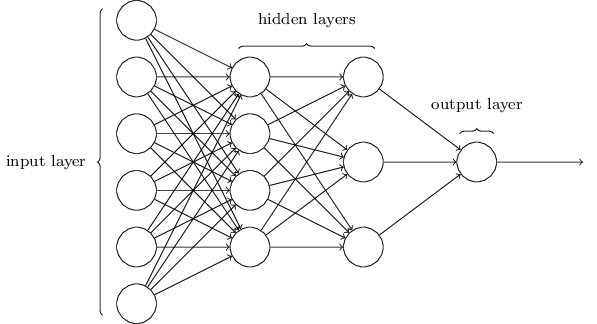
\includegraphics[scale = 0.4]{layers}
\caption{Structure du réseau de neurones}
 
\end{figure}

Le neurone lui-même est composé d'une porte d'entrée qui réalise la combinaison linéaire des sorties des neurones de la couche
précédente qui lui sont connectés, pondérés par les poids associés aux liaisons concernées. Un \textit{bias} peut être ajouté
à la combinaison linéaire; le vecteur composé des \textit{bias} est alors un vecteur lui-même passé en entrée. La valeur obtenue
passe alors dans une fonction seuil. Ici on utilise la sigmoïde $$ \varphi : x \longmapsto \frac{1}{1+\exp(-x)}$$ qui a l'avantage
d'être continûment dérivable. La valeur de sortie du neurone est la valeur qu'on obtient alors.
\begin{figure}[h]
\centering
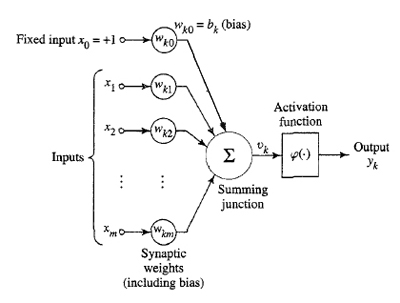
\includegraphics[scale = 0.6]{neuron}
\caption{Neurone}
 
\end{figure}

\section{Résultats}

\section{Discussion}

\section{Conclusion}

\section{Sources}

https://www.google.com/imgres?imgurl=http%3A%2F%2Fneuralnetworksanddeeplearning.com%2Fimages%2Ftikz11.png&imgrefurl=http%3A%2F%2Fneuralnetworksanddeeplearning.com%2Fchap1.html&docid=knJaSo4wqQHuCM&tbnid=NTVnecn7gEka_M%3A&vet=10ahUKEwjw2ceLj4XbAhWELlAKHWYACcAQMwikASgCMAI..i&w=597&h=324&client=ubuntu&bih=647&biw=1301&q=neural%20network&ved=0ahUKEwjw2ceLj4XbAhWELlAKHWYACcAQMwikASgCMAI&iact=mrc&uact=8
https://www.google.com/imgres?imgurl=https%3A%2F%2Fwww.codeproject.com%2FKB%2Fdotnet%2Fpredictor%2Fneuronmodel.jpg&imgrefurl=https%3A%2F%2Fwww.codeproject.com%2FArticles%2F175777%2FFinancial-predictor-via-neural-network&docid=ANecEnYoAqzpQM&tbnid=PKC-AKzH-pbV8M%3A&vet=10ahUKEwjGyd2zjoXbAhVQJFAKHWdJBNYQMwjPASgYMBg..i&w=400&h=303&client=ubuntu&bih=647&biw=1301&q=neural%20network%20neuron&ved=0ahUKEwjGyd2zjoXbAhVQJFAKHWdJBNYQMwjPASgYMBg&iact=mrc&uact=8

\end{document}
